\documentclass[11pt, oneside]{article}
\usepackage{geometry}
\usepackage{graphicx}
\usepackage{amssymb}
\usepackage{epigraph}
\usepackage{amsmath}
\usepackage[doublespacing]{setspace}
\usepackage{etoolbox}
\geometry{letterpaper}

\usepackage[sc]{mathpazo}
\usepackage{eulervm}

\setlength\epigraphwidth{15cm}
\setlength\epigraphrule{0pt}
\makeatletter
\patchcmd{\epigraph}{\@epitext{#1}}{\itshape\@epitext{#1}}{}{}
\makeatother

\title{Exploring methods of quantifying intelligence using theories in Machine Learning}
\author{Abhi Agarwal (abhia@nyu.edu)}
\date{}	

\begin{document}
\maketitle

\par Intelligence has been defined in many different ways, and each of these definitions have allowed us to quantify or understand it in a different way. The simple act of telling an individual how intelligent she is, is the most basic act of quantifying intelligence, which we do in our day-to-day lives. By stating that a particular individual is intelligent we could mean several different things. For example, we could be commenting on their ability to gain knowledge at speed, their accomplishments, their society/community group, their ability to reason, and much more. These are certain characteristics that we, as a society, think about when making a judgement about an individual's intelligence. The most intelligent individuals partake in this by accepting awards for their high IQ or even accept genius grants; even those who may not be as intelligent participate in this by observing this phenomenon and by discussing it. Therefore, there is an inherent part of our society and the way we perceive of the world that needs to compare or judge intelligence.

\par The idea of trying to quantify intelligence or measuring intelligence was first introduced by the field of Phrenology, by Franz Joseph Gall, who is known to be the founder of the field. Gall tried to study the localization of the mental functions in the brain by observing skull sizes and facial features of people. Even though the field of Phrenology was ultimately unsuccessful, some of the concepts such as attempting to quantify intelligence intrigued the scientific community. Moreover, another individual we studied in class that tried to attempt to define intellectual ability was Samuel George Morton. Morton, in his work Crania Americana, claimed that you could measure the intellectual ability of a race by their skull capacity. 

\par This idea become more popular when Alfred Binet and Theodore Simon, in France, designed the first wide-used intelligence test known as the Binet-Simon Scale. Binet personally believed that intelligence is too broad a concept to quantify with a single numerical value. However, he did agree that intelligence is influenced by a number of factors, and can be compared if broken down into its parts. In 1916, the Binet-Simon Scale was brought to Stanford University and researchers adapted it to become the Intelligence Quotient or IQ. The reason for the U.S. to create an intelligence test, as we read in class, was to screen army recruits during World War 1. In addition, IQ tests were also used to screen immigrants as they arrived at Ellis Island, and became increasingly useful to governments as the century progressed. 

\par Throughout the 20th century, the IQ test was used to filter out individuals in different ways. It has been used to determine individuals who would receive prizes and grants, for military and government recruitment, in medicine, job interviews, universities, and much more. We are dependent on ways to quantify intelligence in order to choose particular individuals, and narrow down our search fields in the same way we have used strength or speed. It is also becoming increasingly more important as we move from jobs being in the primary and secondary sector to the tertiary sector. 

\par In the same way, in Computer Science there has been a big push from large organizations to make computers increasingly more intelligent to allow for the reduction of costs. This push, as well as the goal for computer scientists to create artificial life, has driven them to define intelligence. Since the development of computers, there has been a vision of creating an intelligent agent, which is an autonomous entity that is goal driven and uses previous knowledge or learns to reach its goal. The community of individuals studying Artificial Intelligence have had different approaches to solving this problem. 

\par In 2007 W\l{}odzis\l{}aw published a paper on Computational Intelligence, and wrote ``Artificial Intelligence (AI) was the first large scientific community, established already in the mid 1950s, working on problems that require intelligence to be solved" (W\l{}odzis\l{}aw, 1). Intelligence is important to the field because it is an inherent part of building artificial life and is integral in building systems that mimic human life. Most of the Artificial Intelligence community is still debating the ways to solve this problem as building an intelligent agent inherently requires a mathematical or computational definition of intelligence. This is necessary in order for the intelligent agent to learn and be able to make intelligent decisions on its own. Building an intelligent agent requires us to define a program algorithmically that would allow it to act autonomously, and in order to do that, a methodology is needed, which it could follow to learn.

\par Given the limitations in terms of computational power pre-2000, research in building an intelligent agent branched off into two approaches. The first was looking at this problem from a mathematical perspective, and the second was exploring neuroscience and the human anatomy to apply the principles of our own intelligence to the building of an intelligent agent. Building an intelligent agent from a mathematical perspective is looking at features, or aspects of intelligence and trying to model them mathematically, in order to later bring them together into one coherent model. The second approach however, looks at how our cerebral cortex was formed and borrows the architecture and the way neurons make connections between things we learn, and looks to apply the same methodology to learning as our brain does. As we are trying to mimic human beings in creating intelligent agents, the theory of learning from the human brain became a desirable and popular theory in the community. 

\par During the next decade, individuals worked on advancing these fields theoretically until they reached a point where processing power could catch up with their research. The decade gave both the branches time to grow their communities and to improve traction around their work, which created a separation in ideology and the way individuals dealt with the aspects of quantifying intelligence. 

\par In order to understand the task of building an algorithm that allows learning, it needs to be explicitly stated what learning is and how a computer is able to achieve this task. This particular task falls into a field that started within the field of Artificial Intelligence called Machine Learning. ``Machine learning studies computer algorithms for learning things. We might, for instance, be interested in learning to complete a task, or to make accurate predictions, or to behave intelligently" (Schapire, 1). The basic process of Machine Learning is the training of the algorithm. In the training process, the algorithm is fed some data, for example weather data, whilst attaching the details of the outcome. An example of this would be to see if it rained given that the temperature was 4'C and it was cloudy. The algorithm would use past data to make predictions for the future, given a similar scenario. In summary, ``machine learning is about learning to do better in the future based on what was experienced in the past" (Schapire, 1).

\par Prediction is key in Machine Learning because it is not certain that it will rain given the weather conditions outside, but the algorithm returns the most probable outcome. This particular type of algorithm is called a classification algorithm where it uses some detail to classify it into a set number of options: sunny, rainy, etc. A learning algorithm would work in the same way; you would teach it how to react in certain scenarios, as well as their outcomes, and it would be able to associate things you teach it together. Learning algorithms are extremely flexible, and there are many ways to approach them.Defining intelligence mathematically and from a neuroscience point-of-view both approach the problem from a Machine Learning perspective, because this allows us to teach the computer without explicitly having to program it into the computer. Machine Learning can be done in many ways as the basic principle of taking in data and returning a prediction applies across all the Machine Learning algorithms, but what you do in between to find the best prediction is what differentiates the methodology. 

\par The two methodologies I will present next try to quantify intelligence in a different way, and each of these theories have been presented by different types of people and are also taught to different types of students. Students who first learn the mathematical side of machine learning are taught to view intelligence as being able to be represented by building blocks, where these blocks make up the intelligence of a person. On the other hand, students who come from a more biological side to machine learning have experience with understanding intelligence as inherent to the brain, and have an understanding of how the human brain processes this information. Thus, they are drawn towards the neuroscience approach to machine learning. Nowadays, there are an equal number of students from each discipline as mathematicians are usually fixated with trying to solve the mathematical puzzle behind learning, whilst biologists have a passion to simulate and form the human brain.

\par Most individuals who look at Machine Learning and Artificial Intelligence wonder if this is a problem worth solving. Is it required for us to create a framework for intelligence? In Computer Science, it has been a dream of most individuals to create a computer intelligent enough for communication with us. Going forward into the future, many individuals argue that it is useful and important to create such a system, as it would allow us to advance more quickly given that we could train it to learn fields such as Physics and Biology, and allow it to assist us in our research. An intelligent agent could potentially have endless amounts of possibilities as it could encapsulate a significant amount of human knowledge, and be able to run simulations and answer questions. The goal state for researchers is to make a system that would structure and understand all the information that we have, so that we can use it to solve complex problems. In Hawkins' book, `On Intelligence', he points out that ``a basic computer operation is five million times faster than the basic operations in [our brains]!" (Hawkins, 66). The only problem that remains is that we have yet to devise algorithms that are able to make predictions as well as, and as fast as our brain does; trying to understand how to represent and quantify intelligence is the first step towards that goal. 

\par In mathematics an intelligent agent is defined as an agent function (Russell, 33). A percept refers to an intelligent agent?s ``perceptual inputs at any given instant" (Russell, 34), which is basically the perception or view it has at a current moment, and the percept sequence is the ``complete history of everything the agent has ever perceived" (Russell, 34). An agent function can be defined as something that ``maps any given percept sequence to an action" (Russell, 35). Given this information, the aim of Computer Scientists studying it from a mathematical perspective is to design agent functions that take in information, and use the history (as we did in the Machine Learning example) to perform some action. Mathematically we represent a function like this as (Wikipedia, Intelligent agent, Structure of agents):

\begin{equation} \label{eu_eqn}
f\colon P^* \to A
\end{equation}

\noindent Where $P^*$ is the percept sequence, and A is an action that it would predict to occur. The agent function is a very high level concept, but represents an understanding of the process. The input to the agent function would be some type of information, and could be a question, a statement, or a response to something that happens. So our first principle that we must extract in order to make an intelligence framework is the idea that intelligence must be general, and must be able to answer and respond to any input it is given. Warren Smith, an ex-professor at the University of Temple writes that ``[a] primary feature of intelligent entities is a willingness to investigate any kind of mental problem, and an ability to solve, or make progress on, some of them" (Warren, 4). This particular section of the definition means that we have to create a particular function that would make associations between pieces of information, and given any input would be able to use those associations to produce an answer. This is a little biased because it expects there to be an initial ``base of knowledge" (Warren, 5) that exists. 

\par Next, intelligence is something that utilizes existing associations to produce answers. In Mathematics and Computer Science, this is known as the Boolean Satisfiability problem, where it has to be able to determine whether there is an interpretation that satisfies given statements. This particular problem comes from the fear that ``what if the machine has got a giant preprogrammed list of all possible answers to all possible questions, and its mechanism of operation is simply lookup in the list?" (Warren, 5), and so mathematicians have to build systems that follow and understand logic statements. Lastly, the idea that intelligence comes with speed. Which means that ``an `intelligence' [accomplishes] its feats without consuming ridiculously large amounts of time or memory space" (Warren, 5). 

\par It is also important to understand a basic framework for how the processing could occur within the function, and how the data that comes in is actually quantified. The basic process would be to first create an initial knowledge base so the agent function is able to use some underlying knowledge. The construction of this initial knowledge base would depend on Machine Learning methods. Say, for example that we enter in a simple definition of Physics, and some of the underlying characteristics behind it, as text into the initial knowledge base. The knowledge base would then convert these words and underlying concepts into some mathematical representation, such as a linear equation. It would convert it by looking at concepts or ideas that are similar to it, and associate to it - a simple way of doing this would to try to match each word in this text to the text of existing knowledge. Now we are able to start making simple associations just by looking at how close two concepts are, and given the fact that we have the equation of the line for each concept, we can see how close they are. In Machine Learning this idea is called clustering, and can be used in forming the mathematical definition of intelligence. 

\par Once this initial knowledge base is constructed, then the function could potentially take in a question, and try to understand it by comparing it to every single existing piece of knowledge in the knowledge base. Then it would select the pieces of knowledge that represent it the best, and use the underlying concepts behind those to answer the question and make a response. It could use the logical functions defined, in order to take multiple statements to see their outcome, and make a prediction based on those. Although the approach I have defined is far too basic to become a framework for intelligence, it was used as the starting point in many mathematical models that try to define intelligence. 

\par From a quantification aspect, here, the mathematical model reduces each particular piece of knowledge (i.e. piece of text) into a linear equation in order for it to represent and compare the information. This is important to note because we are no longer using the text to represent the piece of knowledge. When you look at more complex frameworks, which involve methods such as gradient-descent or finding global maxima, we would be reducing the importance of the piece of text the particular linear equation represented, and be more fixated on being able to compare it. It would boil down to a single numerical value and decisions about whether the information is related to another piece of knowledge becomes a question of how close they are in numerical value, rather than how we perceive it. This idea introduces several issues that many individuals are opposed to, because here we are not building a system that is intelligent in the same way as us. In addition, there are also individuals who argue that truly-intelligent agents are not possible because no matter how the algorithms are programmed, it comes down to just manipulations of turning a bit on and off. 

\par Moreover, Jeff Hawkins' Intelligence introduces the idea of using the framework of our brain to guide the design of an algorithm. Hawkins utilizes the idea of neurons in our brain as a way to represent one single piece of information. The basic theory behind this is that our brain has millions of neurons, which are connected by synapses. Synapses are how two pieces of information would be connected, and these synapses are basically an edge if we look at this particular problem from a graph perspective while each neuron is a node. Hawkins treats the network of neurons in our brain as an encoding problem, and he quotes ``all your brain knows is patterns" (Hawkins, 56). Each synapse represents a connection, and multiple connections form a pattern. If a particular input was to be put into this graph, then the brain would recognize this input, and try to decipher the pattern the synapses use and the relationships between each neuron. 

\par Hawkins explains that our understanding of the world is based upon patterns and ``[correct] predictions result in understanding. Incorrect predictions result in confusion and prompt you to pay attention" (Hawkins, 89). Most children go through a period where they are trying to learn how to catch a ball. When you are trying to catch a ball the first time, the brain gets a signal to try to recognize a pattern, and as it is the first time, there is no pattern, so you are not successful in catching the ball. Then as the ball is thrown to you again and you try to catch it, the brain figures out the correct motions and patterns your body should make to catch the ball. As you catch the ball more and more, your brain trains itself to perform better because correct predictions result in understanding, whereas incorrect predictions allow the brain to understand that it has made a mistake and it needs to try another pattern in the next attempt. This is a basic description of the way neuroscientists attempt to create learning algorithms that mirror the way we learn.

\par Hawkins', and the neuroscience community's, view of how our brain recognizes patterns and learns is that our ``brain doesn't `compute' the answers to problems; it retrieves the answers from memory ... entire cortex is a memory system. It isn't a computer at all" (Hawkins, 68). Thus, Hawkins sees the brain as being able to predict the answer or the best outcome of a certain task by having a very efficient prediction system that utilizes the connection of neurons in our brain to find the best prediction. The algorithmic technique of doing this is called neural networks. A neural network is an approach where each particular topic is represented by a neuron or a node in a giant graph. The approach is that you have an incoming input, which gets split into a series of inputs that is determined by the algorithm. One approach could be to split the input into individual words. Each word would then be searched as a pattern in the knowledge base, in this case it is called the `Hidden Layer', and if there exists a pattern in the hidden layer then it would do something call ?fire?. Fire is an operation that occurs when it reacts positively to a particular input, and the output is determined by the different types of neurons in the hidden layer that fire. The image shows an example of a neural network, and how it would work below.\footnote{http://www.astroml.org/\_images/fig\_neural\_network\_1.png}

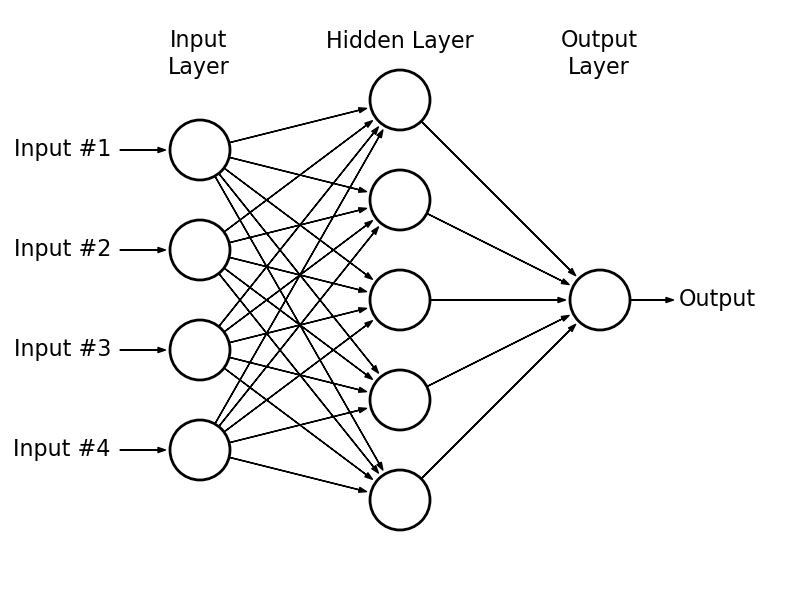
\includegraphics[scale=0.5]{fig_neural_network_1.png}

\par Let us consider an example. Each of the inputs in the image above are sentences that belong to a paragraph. We are trying to give it 4 statements and seeing if they relate or not. The hidden layer allows the algorithm to decide whether it should fire or not, which depends on whether those particular statements are recognized as patterns or not, and depending on if they fire, the output layer gets a response (no response if it does not fire, and there is a response if it does fire). The easiest way to recognize a pattern would be to count the number of responses, and make a judgement at the output layer. If the output layer gets 4 responses, then the paragraph is correct, and if not then it is not. Neural networks are built in this way, but they can have a varying number of inputs, hidden layers (multiple layers as well as more neurons in those layers), and outputs. 

\par The quantification aspect of a neural network is that each particular edge or synapse that exists has to be given a particular weight or quantity that allows it to fire. Even though the information within the knowledge base remains the same, the connections that are established between pieces of information are arbitrary and are not decided by comparing the two methods, but by testing the path that patterns occur in multiple times, and seeing what would produce the best result. We are attempting to simply fine tune the parameters for the neural networks without any regards to what the numerical values represent. These arbitrary values are tested and manipulated in the same way that the brain is trained when we learn to catch a ball. The patterns and connections that are improved by catching it repeatedly depict the same change that occurs, but in this case it is manipulating the weight, or connection value, of a synapse. 

\par A useful and prominent example of the implementation of Machine Learning techniques is Google's intelligent personal assistant ?Google Now?. It uses techniques such as neural networks, that are described by Hawkins above to achieve this goal. Google Now was a breakthrough when it was introduced in the Machine Learning and Artificial Intelligence community. However, it was not a significant breakthrough to the intelligent agents that computer scientists are trying to create. These particular applications are utilizing these technologies, but in specific applications, such as for speech recognition or predictive typing. The particular goal of building an intelligent agent is that it would be able to learn and behave on its own regardless of its application, and it should not be focused and programmed to do something specific. This introduces a new problem; both Jeff Hawkins and Warren Smith have mentioned the issue of generality in the algorithm.

\par The idea that the scientific community is attempting to find a single mathematical definition or a single algorithm that learns or tries to link pieces of information together to form a knowledge base to make predictions, sounds quite absurd. However, we are attempting to do the same things in Physics, and many other fields. In Physics, scientists are trying to find a theory that explains the existence of the universe, and that is what computer scientists, neuroscientists, and mathematicians are attempting to do with the brain. The idea of generality is very important in defining and quantifying intelligence as even IQ tests attempt to highlight test for general intelligence (g factor). 

\par After understanding these approaches, the question we have to answer becomes: Is quantifying intelligence using the framework of our brain any better than quantifying intelligence using mathematics? It seems a little confusing, but because we are attempting to replicate something we would call truly intelligent, our brain, does the methodology we follow become a better approach than defining it mathematically? The idea is that we are still unsure how our brain processes or even `stores' things we know, thus it becomes difficult to understand if it is a problem to quantify something that should not be quantified. Intelligence is a construct that we have created to define certain characteristics that an individual has, but it is a construct that is slowly being supported by scientific evidence. 

\par However, there are arguments against using our brains as a framework for intelligence. Firstly, understanding things we look at is a particular of intelligence- not the process of being able to see things, but the process of looking at particular items and being able to comprehend them (the same extends to all senses). Vision in Computer Science is studied in the field of Computer Vision, and in Computer Vision there exists a problem: when you try to develop Machine Learning algorithms that mirror the way we think, things like optical illusions become a problem for it. Because the computer is trained and taught to learn things the same way we do, and perceives the contents on a page or a screen in the same way as us, it too faces the same problems and limitations our brains do. 

\par In conclusion, generality is important when defining intelligence and building intelligent agents. Building an intelligent agent requires knowledge or information to be quantified and manipulated without regards to what its primary meaning is, but this is a trade-off we have to accept. Quantifying intelligence is becoming increasingly important in our society as we have increased our reliance on building tests or tools that require us to understand intelligence and there is a push to move towards building tools that are truly intelligent.

\begin{thebibliography}{9}
\bibitem{1}
	Hawkins, Jeff, and Sandra Blakeslee,
	\emph{On Intelligence}.
	New York: Henry Holt, 2005.
	Print.
\bibitem{2}
	Duch, W\l{}odzis\l{}aw.
	\emph{"What Is Computational Intelligence and What Could It Become?" Challenges for Computational Intelligence.}
	2007: n. pag. Print.
\bibitem{3}
	Schapire, Rob. 
	\emph{Theoretical Machine Learning.} 
	(n.d.): n. pag. COS 511: Theoretical Machine Learning. Princeton University. 
	Web.
\bibitem{4}
	Russell, Stuart J., Peter Norvig, and John F. Canny. 
	\emph{Artificial Intelligence : A Modern Approach.}
	Upper Saddle River: Pearson Plc, 1999. Print.
\bibitem{5}
	Wikipedia, the Free Encyclopedia. 
	\emph{Intelligent agent}.
	N.p., n.d. $<$http://en.wikipedia.org/wiki/Intelligent\_agent$>$.
	Web.
\bibitem{6}
	Smith, Warren D. 
	\emph{Mathematical Definition of ``Intelligence"}.
	Indiana U, 2006. Abstract. University of Indiana. N.p., 18 July 2006. 
	Web.
\end{thebibliography}
\end{document}  